\documentclass[11pt]{article}

\usepackage[margin=1in]{geometry}
\usepackage[T1]{fontenc}
\usepackage[utf8]{inputenc}
\usepackage{lmodern}
\usepackage{microtype}
\usepackage{amsmath,amssymb,mathtools}
\usepackage{hyperref}
\usepackage{graphicx}
\usepackage{subcaption}
\usepackage{float}
\hypersetup{hidelinks}

\title{Meeting notes on preconditioned operator GD on $S^1$}
\author{Shreyas Kalvankar}
\date{\today}

\begin{document}
\maketitle

\section*{Summary}

We study whether a low-frequency Fourier-block preconditioner can reduce the
difference in convergence rates across modes for kernel/operator gradient descent on $S^1$.
We compare three flows:
\[
	\text{baseline: } B=A,
	\qquad
	\text{theory-preconditioned: } B=B_{\mathrm{th}},
	\qquad
	\text{empirical-preconditioned: } B=B_{\mathrm{emp}}.
\]
Here $A=K/n$ is the normalized empirical operator, $B_{\mathrm{th}}$ is built
from the finite-$n$ eigenvalue matrix $\Lambda^{(n)}$, and
$B_{\mathrm{emp}}$ is built from the actual sampled low-frequency block $C$.

The main conclusions are:

\begin{enumerate}
	\item For a low-frequency target, both preconditioned flows make the active
	      low-mode residual curves much more similar than in the baseline, and
	      the theory-based construction is already very close to the empirical one.

	\item In function space, the low-frequency target is fitted almost perfectly
	      by both preconditioned flows, while the baseline leaves a visibly larger residual.

	\item For a target with additional higher-frequency components outside the
	      retained block, the preconditioner still helps a lot on the retained
	      modes, but it cannot fully remove the error coming from frequencies
	      outside that block.
\end{enumerate}

\section*{1. Setup and objects}

We parameterize the circle by $\gamma \in [0,2\pi)$ and embed it as
\[
	x(\gamma)=(\cos\gamma,\sin\gamma).
\]
For each run, we sample training angles
\[
	\gamma_1,\dots,\gamma_n \overset{\mathrm{iid}}{\sim} \mathrm{Unif}[0,2\pi),
\]
build the analytic circle kernel matrix
\[
	K_{ij}=\Theta(\gamma_i,\gamma_j),
\]
and define the normalized empirical operator
\[
	A=\frac{1}{n}K.
\]

To isolate low-frequency structure, we form the real Fourier block up to
frequency $K_{\max}$:
\[
	\phi_0(\gamma)=1,
\]
\[
	\phi_{k,c}(\gamma)=\sqrt{2}\cos(k\gamma),
	\qquad
	\phi_{k,s}(\gamma)=\sqrt{2}\sin(k\gamma),
	\qquad k=1,\dots,K_{\max}.
\]
Evaluating these functions on the sampled training angles gives
\[
	\Phi \in \mathbb{R}^{n\times d},
	\qquad
	d=2K_{\max}+1.
\]

The main sampled low-block objects are
\[
	G=\frac{1}{n}\Phi^\top\Phi,
	\qquad
	H=\frac{1}{n}\Phi^\top A\Phi,
	\qquad
	C=G^{-1}H.
\]
Here $C$ is the empirical operator written in sampled Fourier coordinates.

The finite-$n$ theory benchmark is the diagonal matrix
\[
	\Lambda^{(n)}=\mathrm{diag}(\lambda_p^{(n)}),
\]
with
\[
	\lambda_p^{(n)}
	=
	\left(1-\frac{1}{n}\right)\lambda_{k_p}
	+
	\frac{1}{n}g(0),
	\qquad
	g(0)=\Theta(x,x).
\]

We compare two preconditioners:

\paragraph{Theory preconditioner.}
\[
	M_{\mathrm{th}}=(\Lambda^{(n)})^{-1},
	\qquad
	P_{\mathrm{th}}=\frac{1}{n}\Phi M_{\mathrm{th}} G^{-1}\Phi^\top,
	\qquad
	B_{\mathrm{th}}=P_{\mathrm{th}}A.
\]

\paragraph{Empirical preconditioner.}
\[
	M_{\mathrm{emp}}=(C+\mathrm{reg}\,I)^{-1},
	\qquad
	P_{\mathrm{emp}}=\frac{1}{n}\Phi M_{\mathrm{emp}} G^{-1}\Phi^\top,
	\qquad
	B_{\mathrm{emp}}=P_{\mathrm{emp}}A.
\]

We use this form because the whole idea is to correct the dynamics only on the
retained Fourier block, rather than trying to invert the full empirical operator.

The training dynamics are
\[
	y_{t+1}=y_t-\eta B\,r_t,
	\qquad
	r_t=y_t-y^*,
\]
with $B=A$, $B_{\mathrm{th}}$, or $B_{\mathrm{emp}}$ depending on the flow.

To compare rates, we project the residual onto the sampled Fourier columns and
normalize by the initial magnitude. If $\phi_p^{\mathrm{unit}}$ is the
sample-normalized $p$-th basis vector, then
\[
	\alpha_p(t)=\langle r_t,\phi_p^{\mathrm{unit}}\rangle,
	\qquad
	\text{mode curve}_p(t)=\frac{|\alpha_p(t)|}{|\alpha_p(0)|}.
\]
These normalized residual mode curves are the main quantity we look at.

\section*{2. Experiment 1: low-frequency target}

For the first experiment we use
\[
	K_{\max}=4,
\]
and the target
\[
	f_{\mathrm{low}}^*(\gamma)
	=
	1
	+0.9\cos(\gamma)
	+0.5\cos(2\gamma)
	+0.35\cos(3\gamma).
\]
So all active target frequencies lie inside the retained low-frequency block.

\subsection*{2.1 Residual mode decay}

Figure~\ref{fig:low-all-modes} shows the normalized residual mode curves,
aggregated over seeds, for the retained cosine modes.

\begin{figure}[H]
	\centering
	
\includegraphics[width=\textwidth]{images/target-low-frequency/all_mode_decay_three_panel_mean_std_n4096.png}
	\caption{Low-frequency target. Mean $\pm$ standard deviation across seeds for the normalized residual mode curves at $n=4096$. The baseline flow shows clear differences between modes, while both preconditioned flows make the low-mode rates much more similar.}
	\label{fig:low-all-modes}
\end{figure}

This is the simplest case for the method. Since the target is entirely inside the
retained block, one expects the low-block preconditioner to make the active
modes decay on more similar time scales. That is exactly what we see: the
baseline keeps clear separation across modes, while both preconditioned flows
bring the active curves much closer together. The theory-based construction is
already very close to the empirical one.

\subsection*{2.2 Function-space fit}

Figure~\ref{fig:low-probe-fit} compares the final probe-grid predictions to the
target.

\begin{figure}[H]
	\centering
	
\includegraphics[width=\textwidth]{images/target-low-frequency/probe_target_vs_prediction_three_panel_mean_std_n4096.png}
	\caption{Low-frequency target. Final prediction on a dense probe grid, shown as mean $\pm$ standard deviation across seeds. Both preconditioned flows are almost indistinguishable from the target, while the baseline leaves a larger smooth residual error.}
	\label{fig:low-probe-fit}
\end{figure}

The same picture appears at the level of the fitted function. The preconditioned
flows do not just change coefficients; they also give a visibly better final fit.
Again, the empirical version only improves slightly over the theory version,
which suggests that $\Lambda^{(n)}$ is already a good approximation to the
sampled low block in this regime.

\section*{3. Experiment 2: mixed / high-frequency target}

For the second experiment we enlarge the retained block to
\[
	K_{\max}=8,
\]
and use the target
\begin{align*}
	f_{\mathrm{high}}^*(\gamma)
	 & =
	1
	+0.9\cos(\gamma)
	+0.5\cos(2\gamma)
	-0.35\sin(3\gamma) \\
	 & \quad
	+0.25\cos(7\gamma)
	-0.10\sin(10\gamma)
	+0.08\cos(12\gamma)
	-0.04\sin(15\gamma).
\end{align*}

The important point is that the retained block stops at frequency $8$, while the
target also contains frequencies $10$, $12$, and $15$. So this is not a best-case
experiment for the preconditioner. The question is whether it still helps on the
retained part of the dynamics, and how much of the remaining error comes from
frequencies outside the block.

\subsection*{3.1 Residual mode decay}

Figure~\ref{fig:high-all-modes} shows the retained active low-block modes for
this target: the constant mode, $\cos(\gamma)$, $\cos(2\gamma)$, $\sin(3\gamma)$,
and $\cos(7\gamma)$.

\begin{figure}[H]
	\centering
	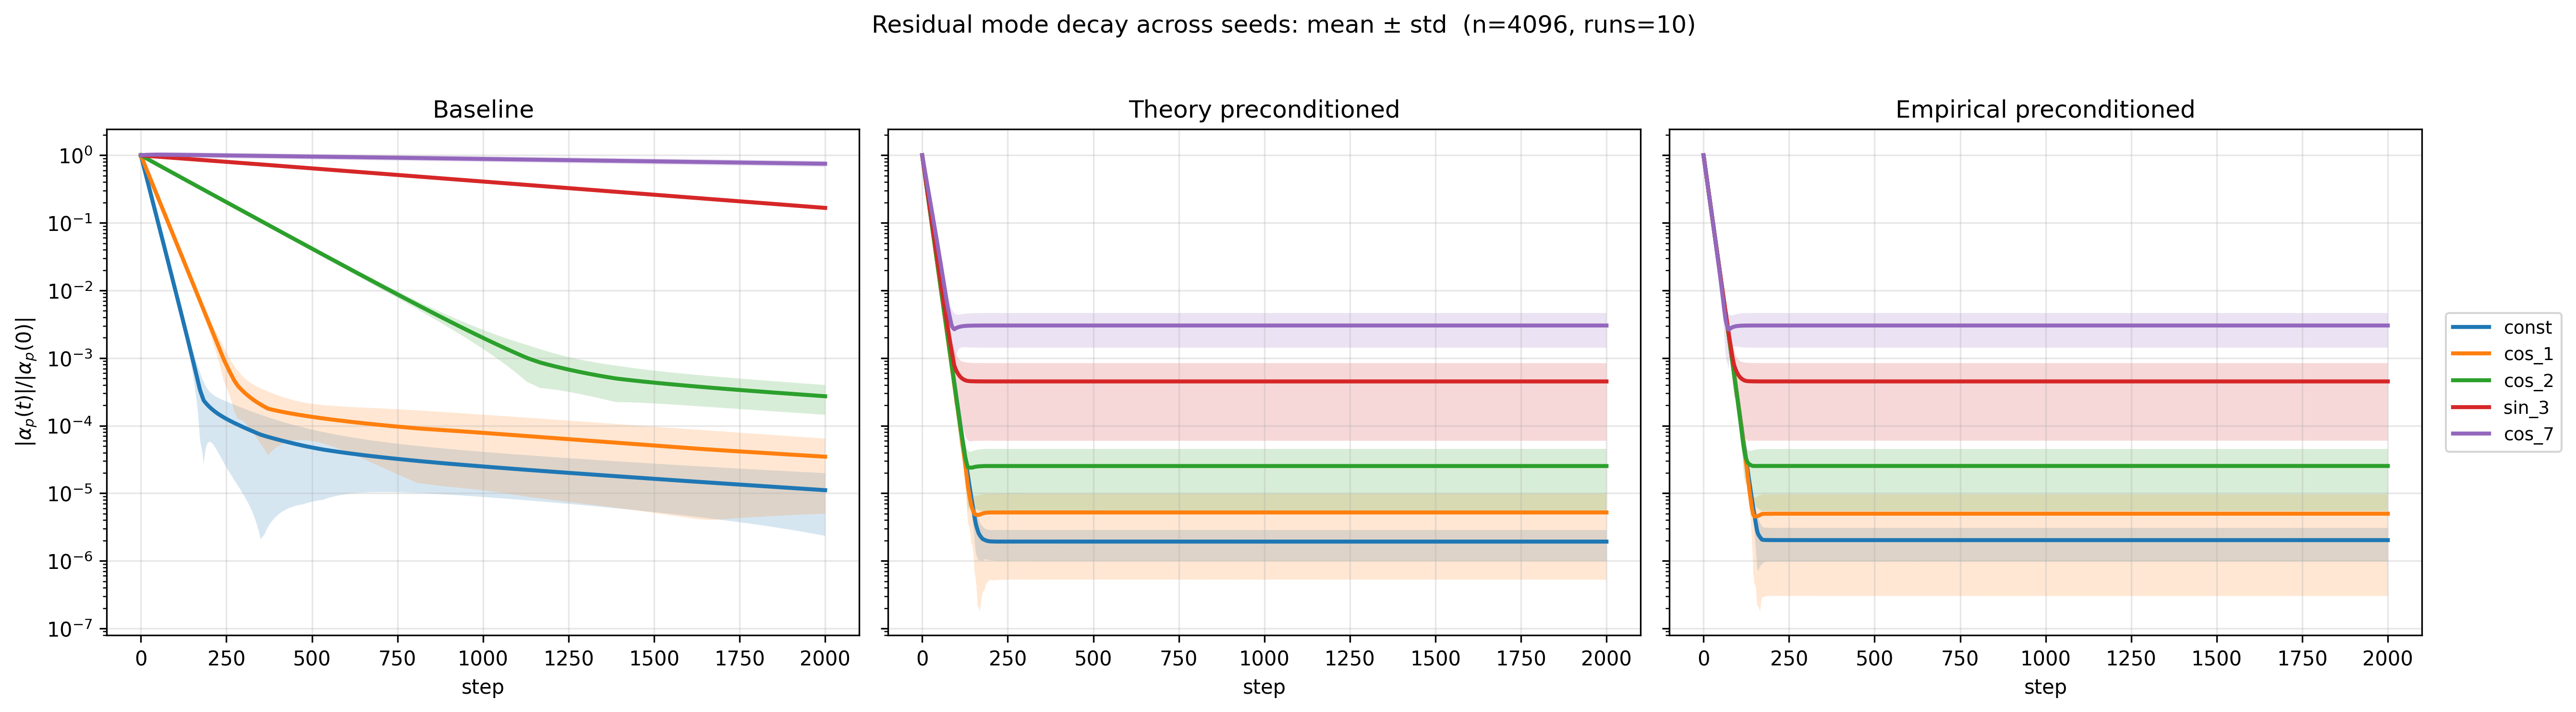
\includegraphics[width=\textwidth]{images/target-high-frequency/all_mode_decay_three_panel_mean_std_n4096.png}
	\caption{Mixed/high-frequency target. Mean $\pm$ standard deviation across seeds for the normalized residual mode curves at $n=4096$. The baseline keeps a strong separation between the retained active modes, while both preconditioned flows make the in-block dynamics much more similar.}
	\label{fig:high-all-modes}
\end{figure}

The interpretation here is different from the low-frequency case. We should not
expect a low-block preconditioner to remove the full difficulty of the target,
because part of the target lies outside the retained block. Even so, the gain is
clear: the retained active modes are brought much closer together, and the
empirical preconditioner remains very close to the theory-based one.

\subsection*{3.2 Function-space fit}

Figure~\ref{fig:high-probe-fit} shows the final probe-grid predictions.

\begin{figure}[H]
	\centering
	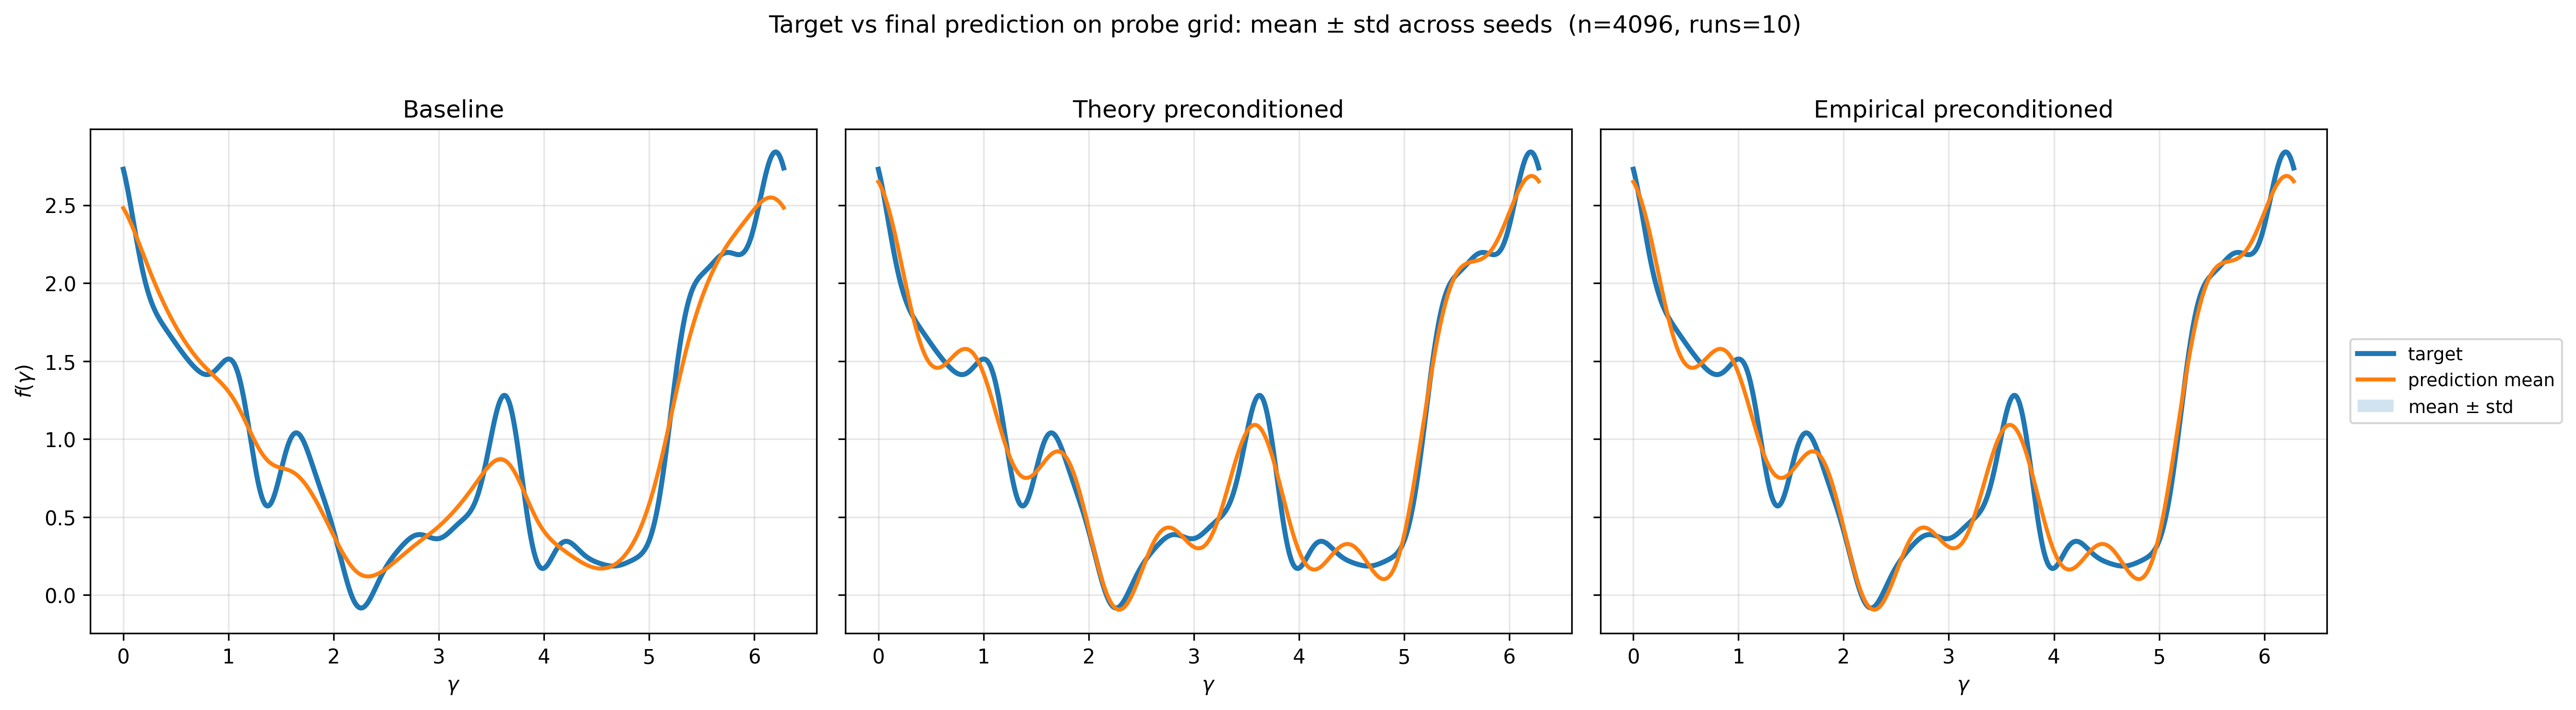
\includegraphics[width=\textwidth]{images/target-high-frequency/probe_target_vs_prediction_three_panel_mean_std_n4096.png}
	\caption{Mixed/high-frequency target. Final prediction on the dense probe grid, shown as mean $\pm$ standard deviation across seeds. Both preconditioned flows improve visibly over the baseline, but they do not remove all of the structured mismatch.}
	\label{fig:high-probe-fit}
\end{figure}

This is what one should expect in the harder setting. The preconditioner still
helps, but the final prediction is not almost exact as in the low-frequency case.
The remaining mismatch is consistent with the target containing frequencies that
are outside the retained block.

\section*{4. Main takeaways}

\begin{enumerate}
	\item The key object is the sampled low-frequency block
	      \[
		      C=G^{-1}H,
		      \qquad
		      G=\frac{1}{n}\Phi^\top\Phi,
		      \qquad
		      H=\frac{1}{n}\Phi^\top A\Phi.
	      \]
	      The empirical preconditioner uses $C$ directly, while the theory
	      preconditioner replaces it by the eigenvalue matrix with diagonal correction
	      $\Lambda^{(n)}$.

	\item In the low-frequency target experiment, the theory preconditioner already
	      behaves very close to the empirical one. This suggests that the
	      finite-$n$ eigenvalue matrix captures the relevant low-block geometry
	      well enough for this purpose.

	\item In the mixed/high-frequency experiment, the right interpretation is more
	      limited. Since the target contains frequencies outside the retained
	      block, one should expect only partial equalization: the preconditioner
	      can help on the retained part, but not directly on the rest.

	\item Overall, these experiments support the view that the preconditioned flow
	      is a correction on the low Fourier block, not an inverse of the full
	      empirical operator.
\end{enumerate}

\clearpage
\appendix

\section*{Supplementary plots: low-frequency target}

The following single-run mode-comparison plots make the rate changes more explicit
for the low-frequency target.

\begin{figure}[H]
	\centering
	\begin{subfigure}[t]{0.48\textwidth}
		\centering
		
\includegraphics[width=\linewidth]{images/target-low-frequency/mode_curve_compare_const_n4096_seed0.png}
		\caption{const}
	\end{subfigure}
	\hfill
	\begin{subfigure}[t]{0.48\textwidth}
		\centering
		
\includegraphics[width=\linewidth]{images/target-low-frequency/mode_curve_compare_cos_1_n4096_seed0.png}
		\caption{$\cos(\gamma)$}
	\end{subfigure}

	\vspace{0.6em}

	\begin{subfigure}[t]{0.48\textwidth}
		\centering
		
\includegraphics[width=\linewidth]{images/target-low-frequency/mode_curve_compare_cos_2_n4096_seed0.png}
		\caption{$\cos(2\gamma)$}
	\end{subfigure}
	\hfill
	\begin{subfigure}[t]{0.48\textwidth}
		\centering
		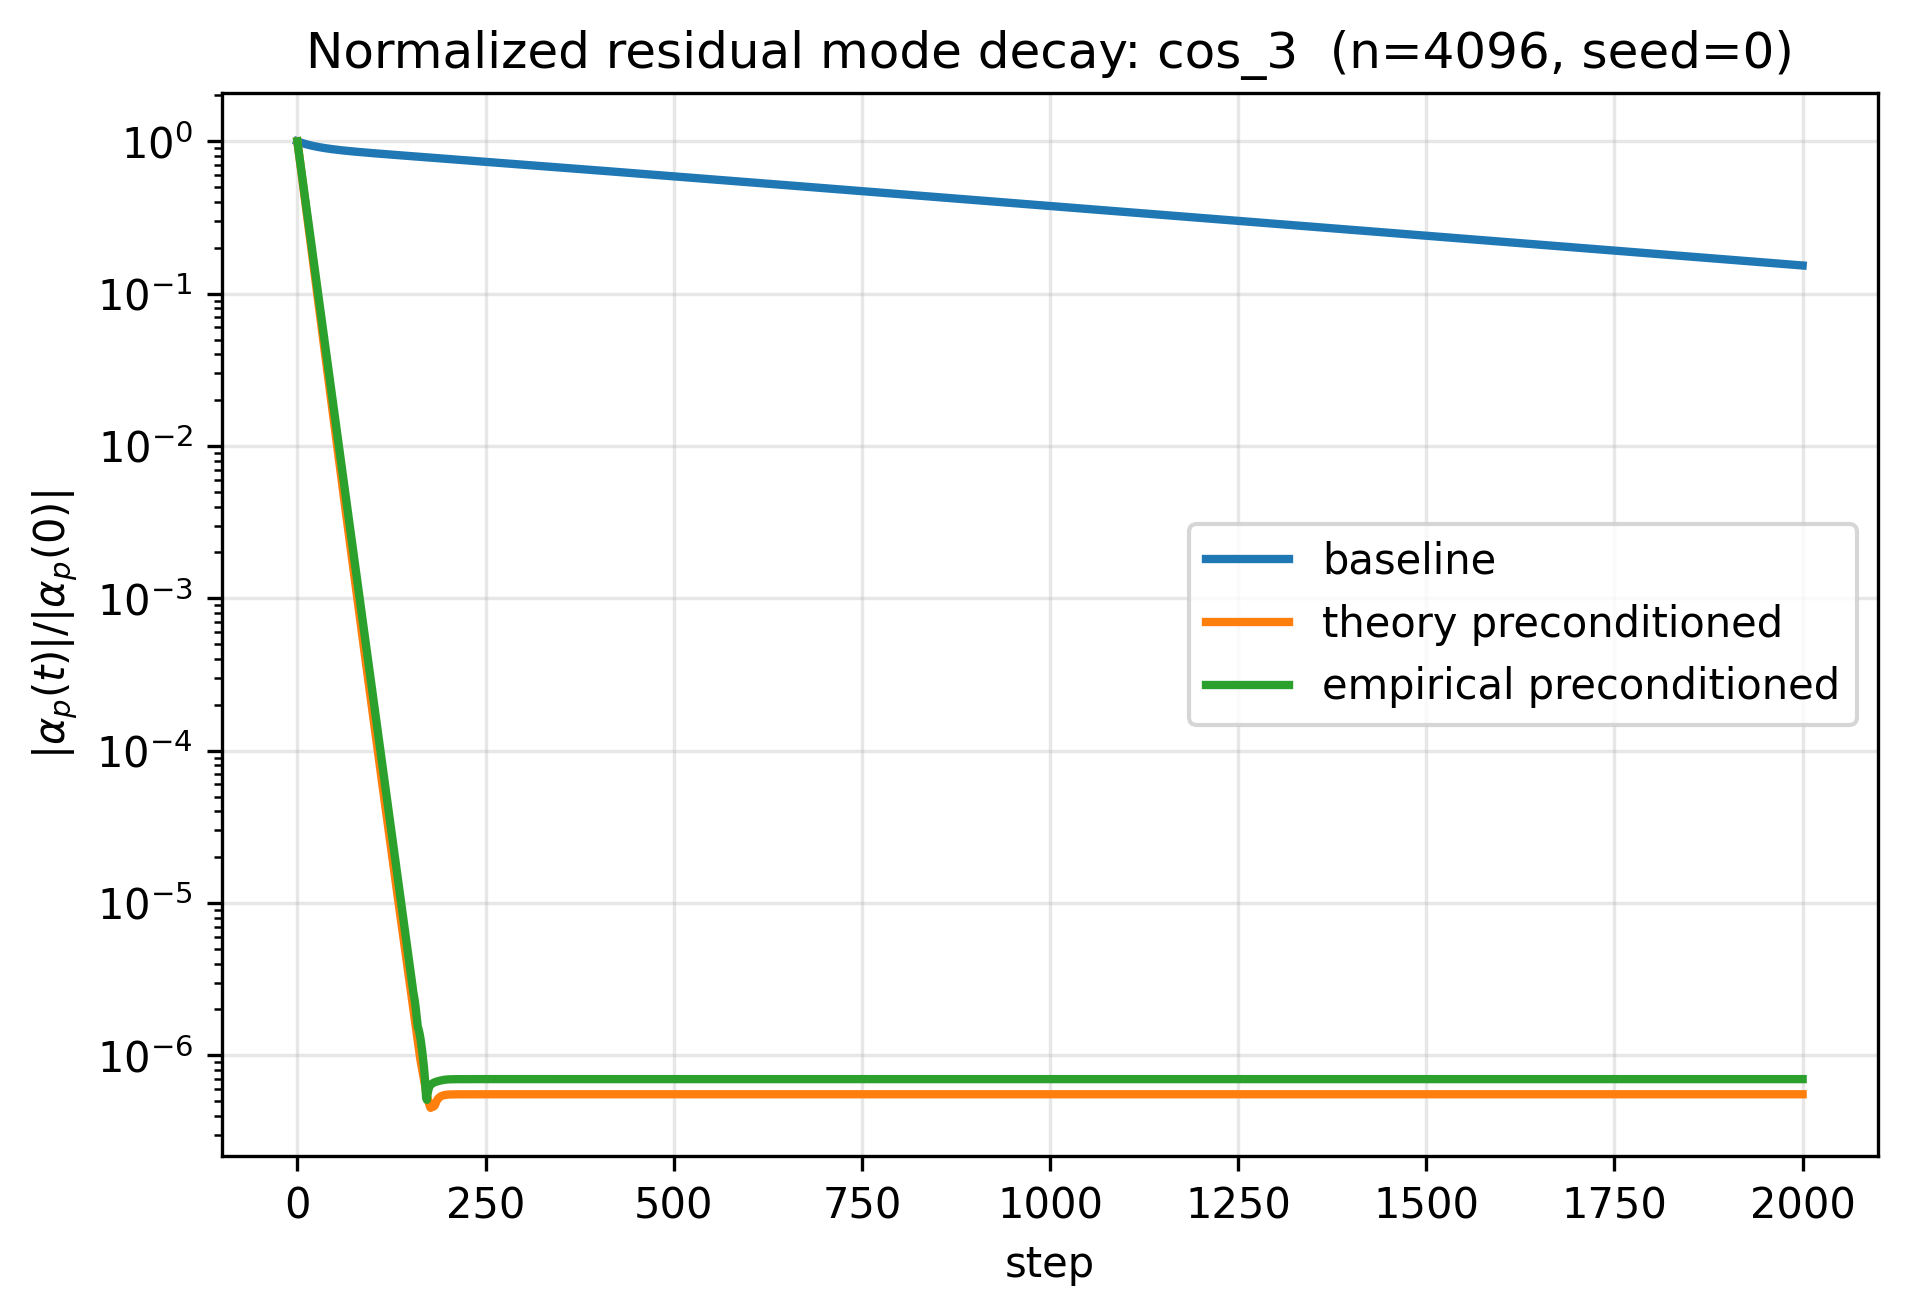
\includegraphics[width=\linewidth]{images/target-low-frequency/mode_curve_compare_cos_3_n4096_seed0.png}
		\caption{$\cos(3\gamma)$}
	\end{subfigure}

	\vspace{0.6em}

	\begin{subfigure}[t]{0.62\textwidth}
		\centering
		
\includegraphics[width=\linewidth]{images/target-low-frequency/mode_curve_compare_cos_4_n4096_seed0.png}
		\caption{$\cos(4\gamma)$}
	\end{subfigure}
	\caption{Low-frequency target. Representative single-run mode comparisons at $n=4096$. The baseline keeps clear differences between modes, while the theory and empirical preconditioners are very close mode by mode.}
\end{figure}

\section*{Supplementary plots: mixed / high-frequency target}

The following single-run plots show the retained active modes for the
mixed/high-frequency target, together with one representative inactive in-block
mode, $\cos(4\gamma)$.

\begin{figure}[H]
	\centering
	\begin{subfigure}[t]{0.48\textwidth}
		\centering
		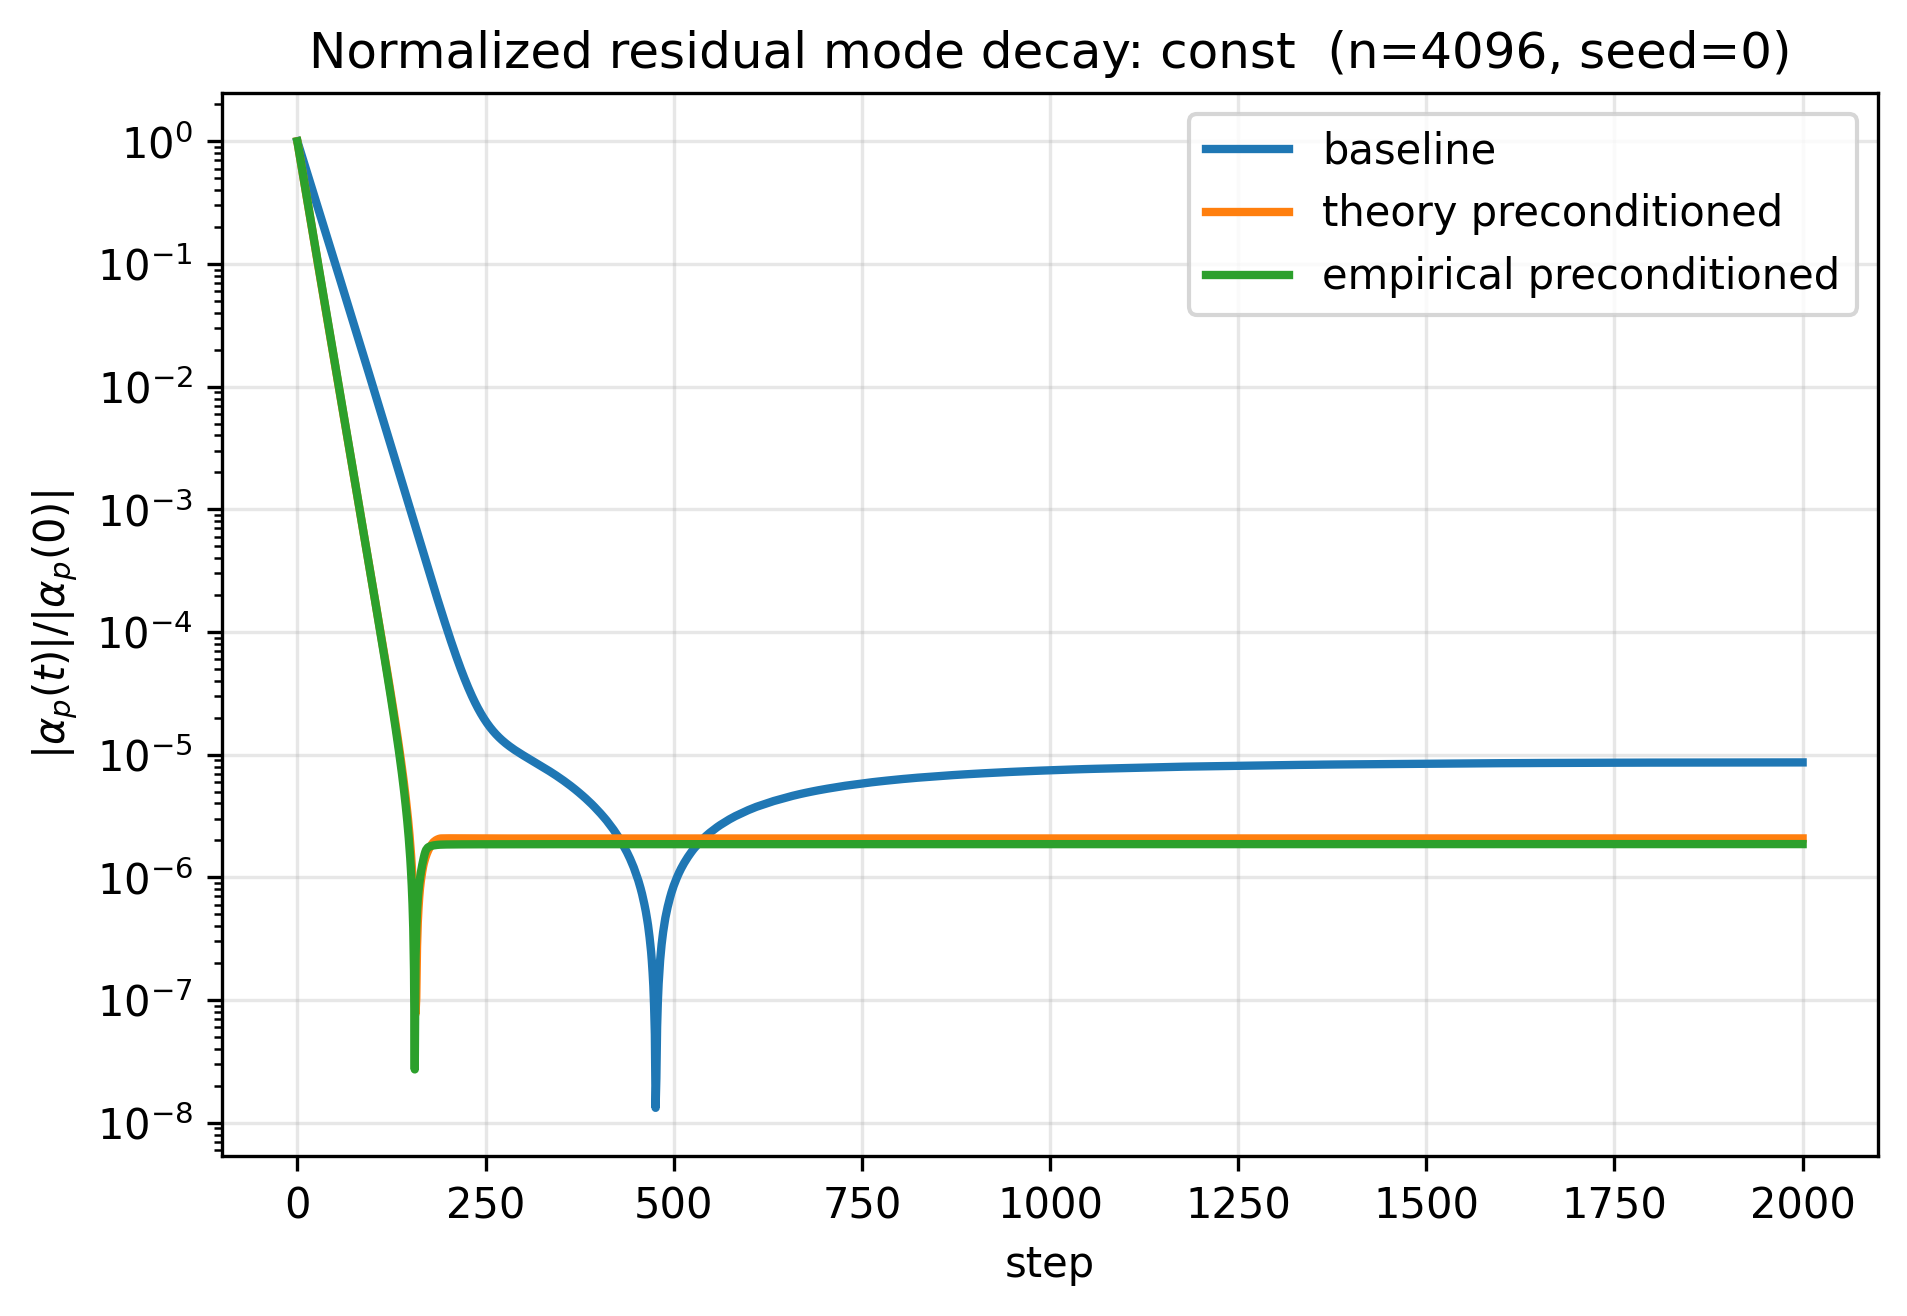
\includegraphics[width=\linewidth]{images/target-high-frequency/mode_curve_compare_const_n4096_seed0.png}
		\caption{const}
	\end{subfigure}
	\hfill
	\begin{subfigure}[t]{0.48\textwidth}
		\centering
		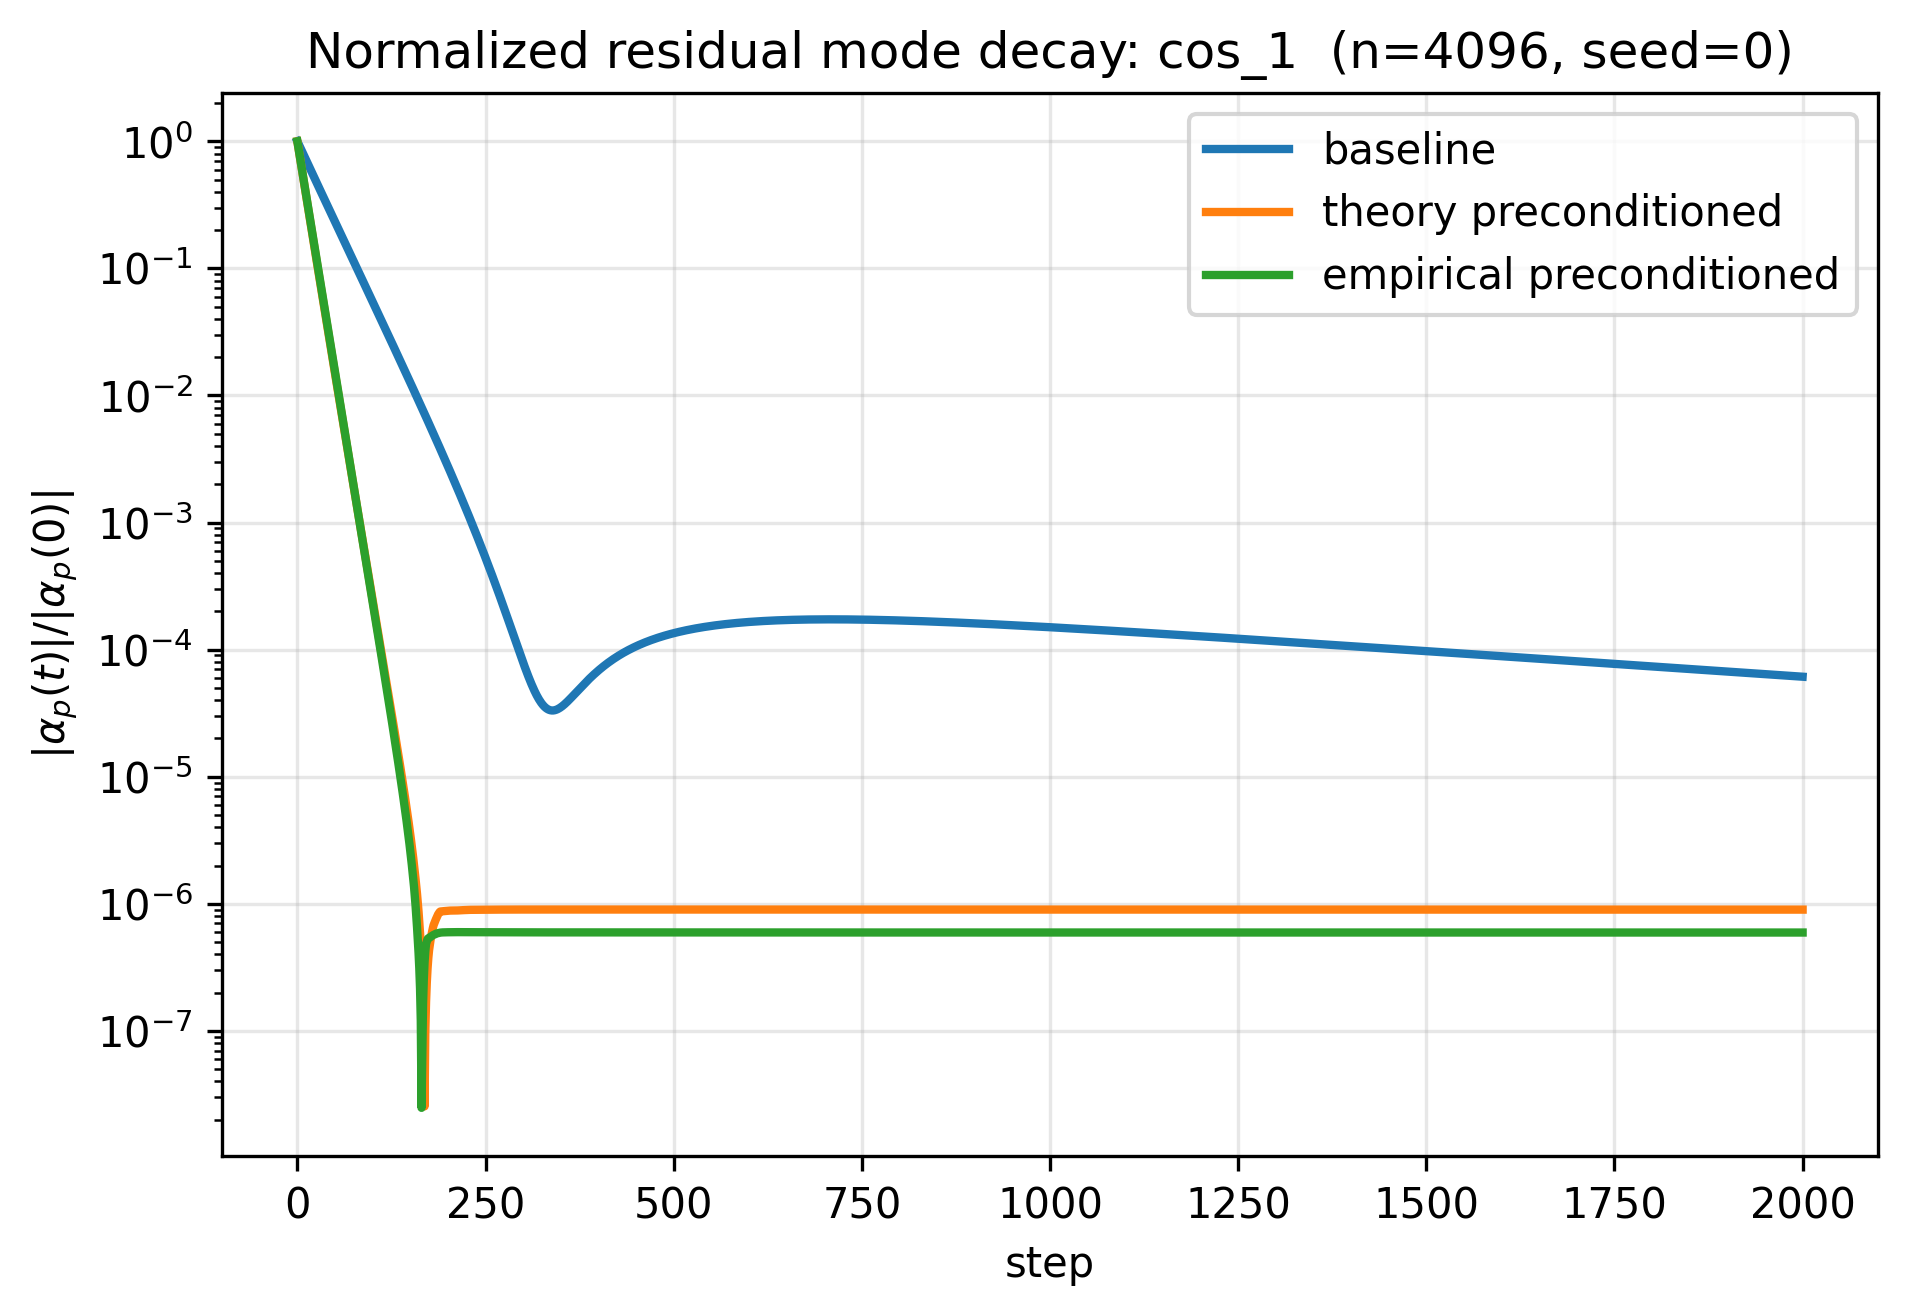
\includegraphics[width=\linewidth]{images/target-high-frequency/mode_curve_compare_cos_1_n4096_seed0.png}
		\caption{$\cos(\gamma)$}
	\end{subfigure}

	\vspace{0.6em}

	\begin{subfigure}[t]{0.48\textwidth}
		\centering
		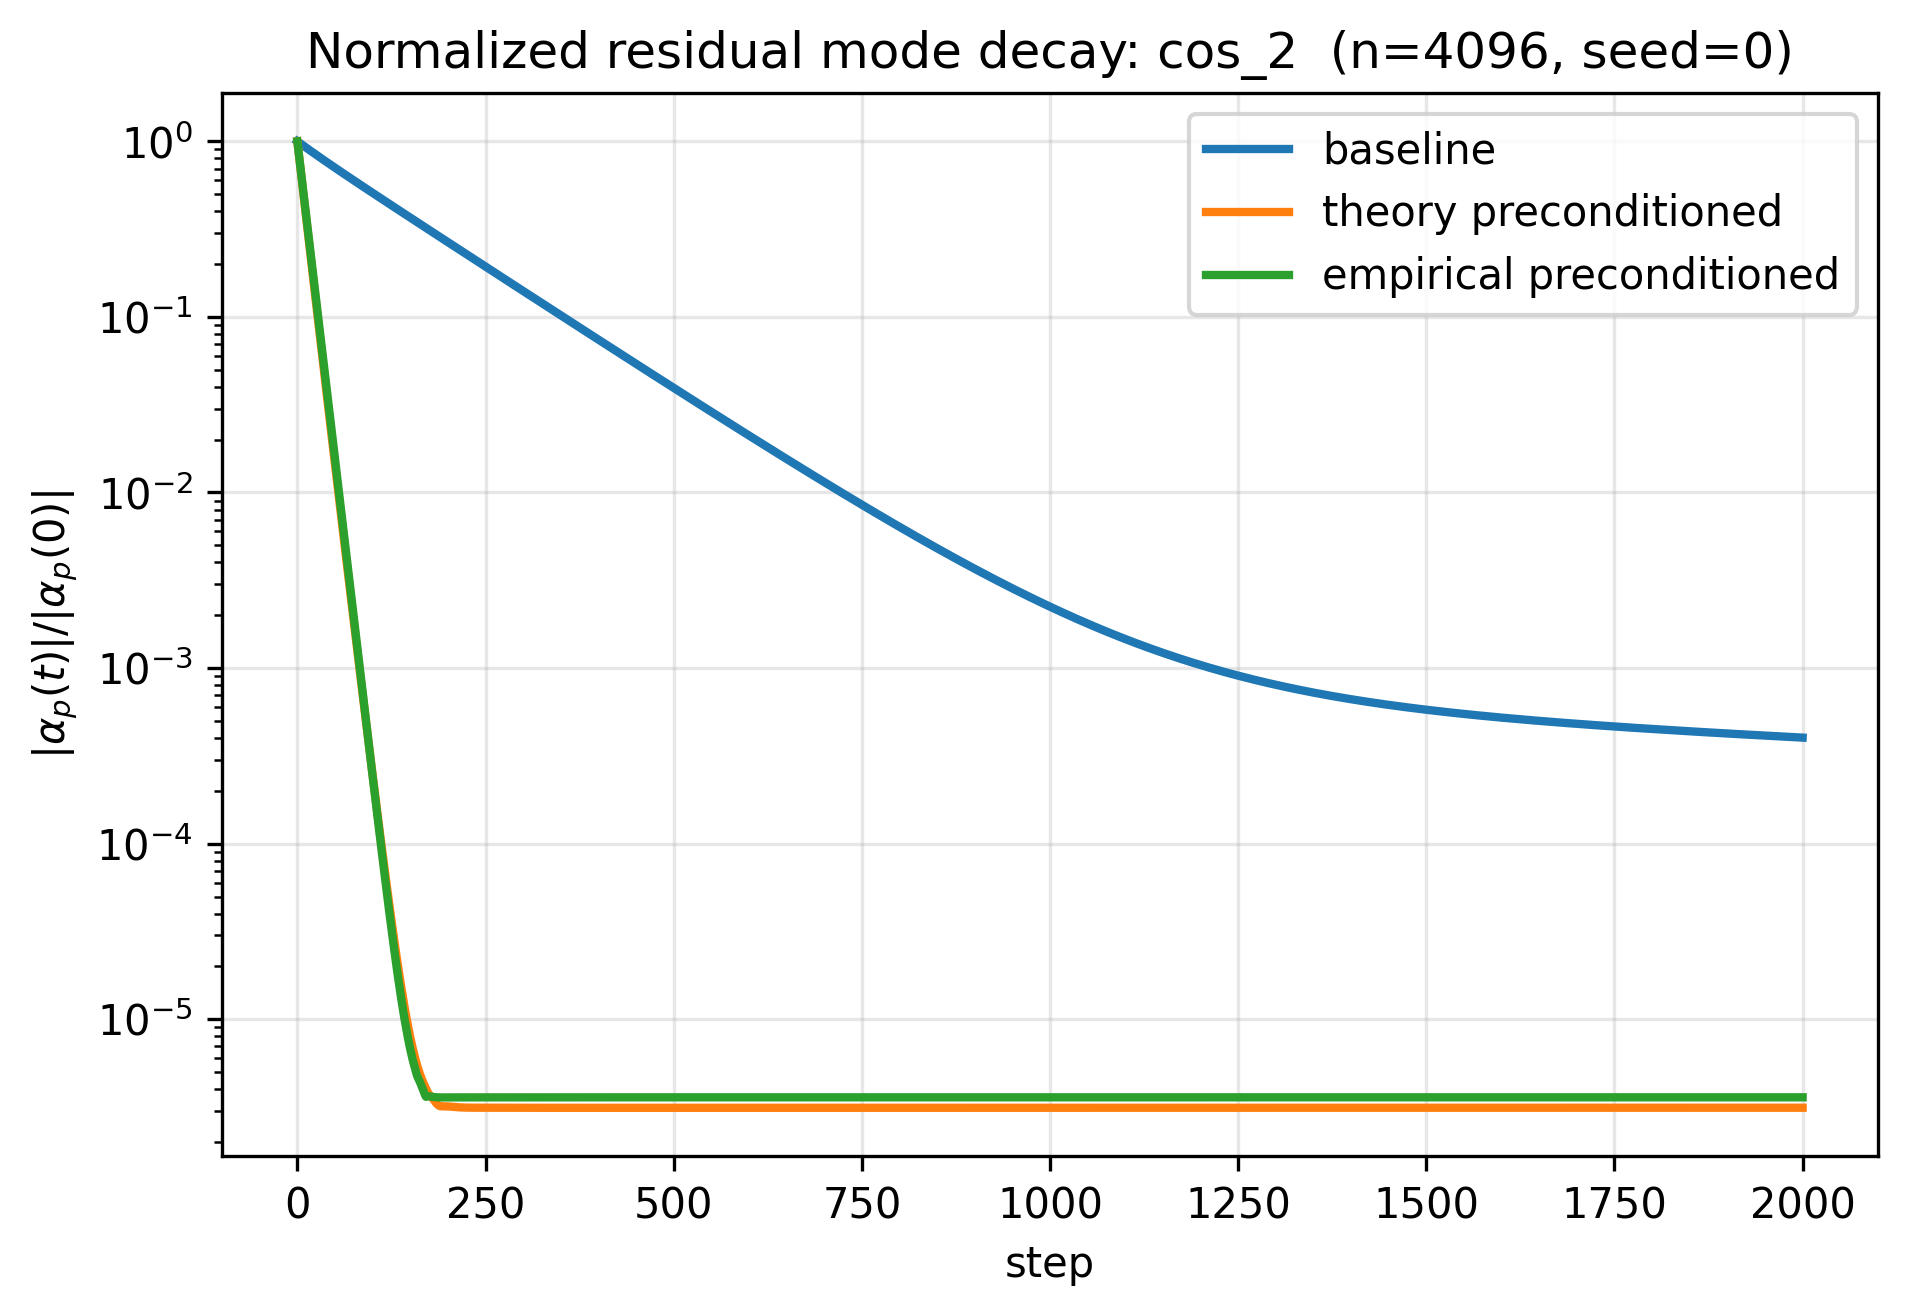
\includegraphics[width=\linewidth]{images/target-high-frequency/mode_curve_compare_cos_2_n4096_seed0.png}
		\caption{$\cos(2\gamma)$}
	\end{subfigure}
	\hfill
	\begin{subfigure}[t]{0.48\textwidth}
		\centering
		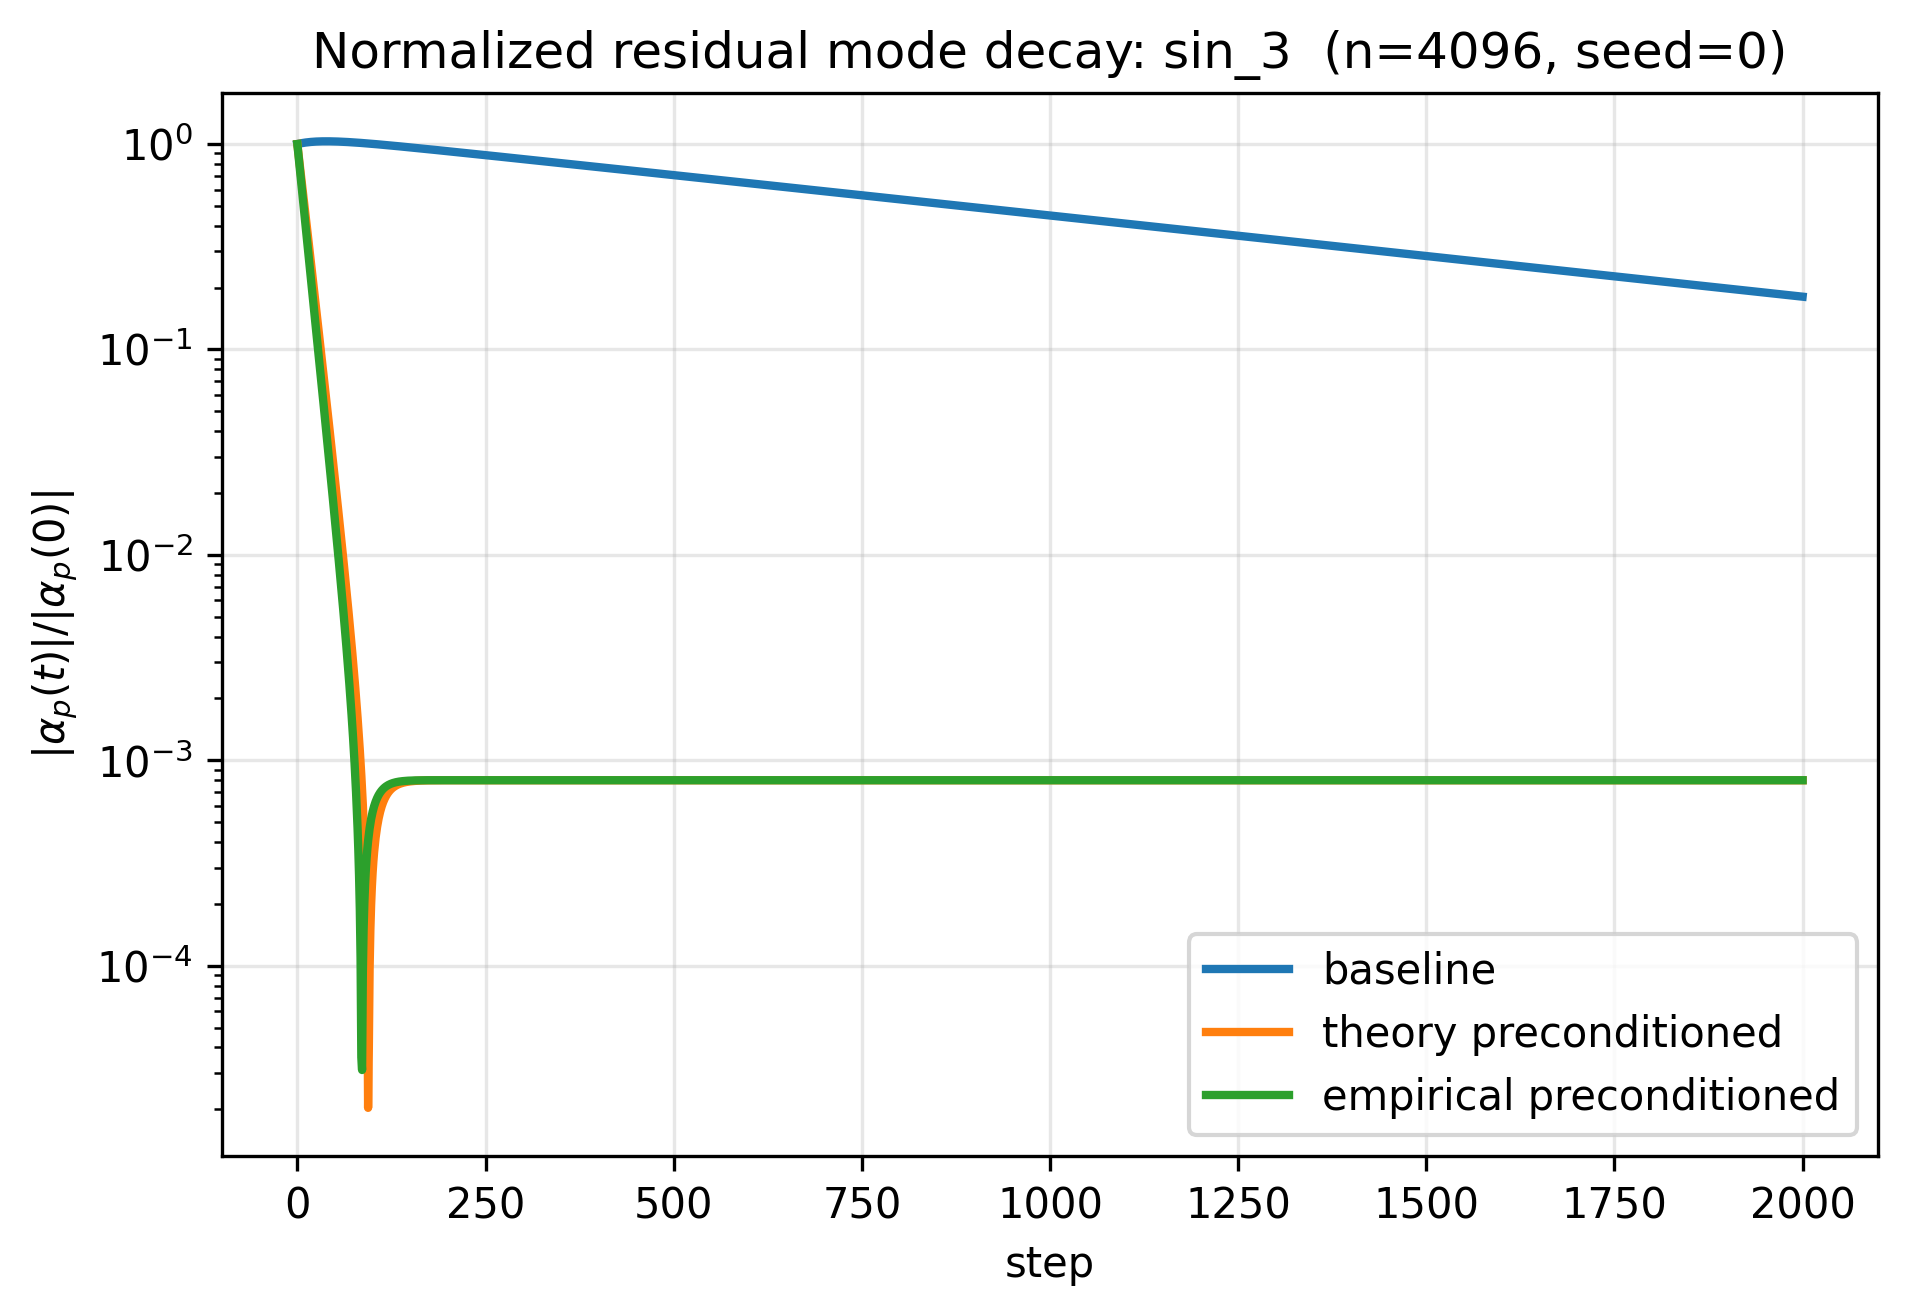
\includegraphics[width=\linewidth]{images/target-high-frequency/mode_curve_compare_sin_3_n4096_seed0.png}
		\caption{$\sin(3\gamma)$}
	\end{subfigure}

	\vspace{0.6em}

	\begin{subfigure}[t]{0.48\textwidth}
		\centering
		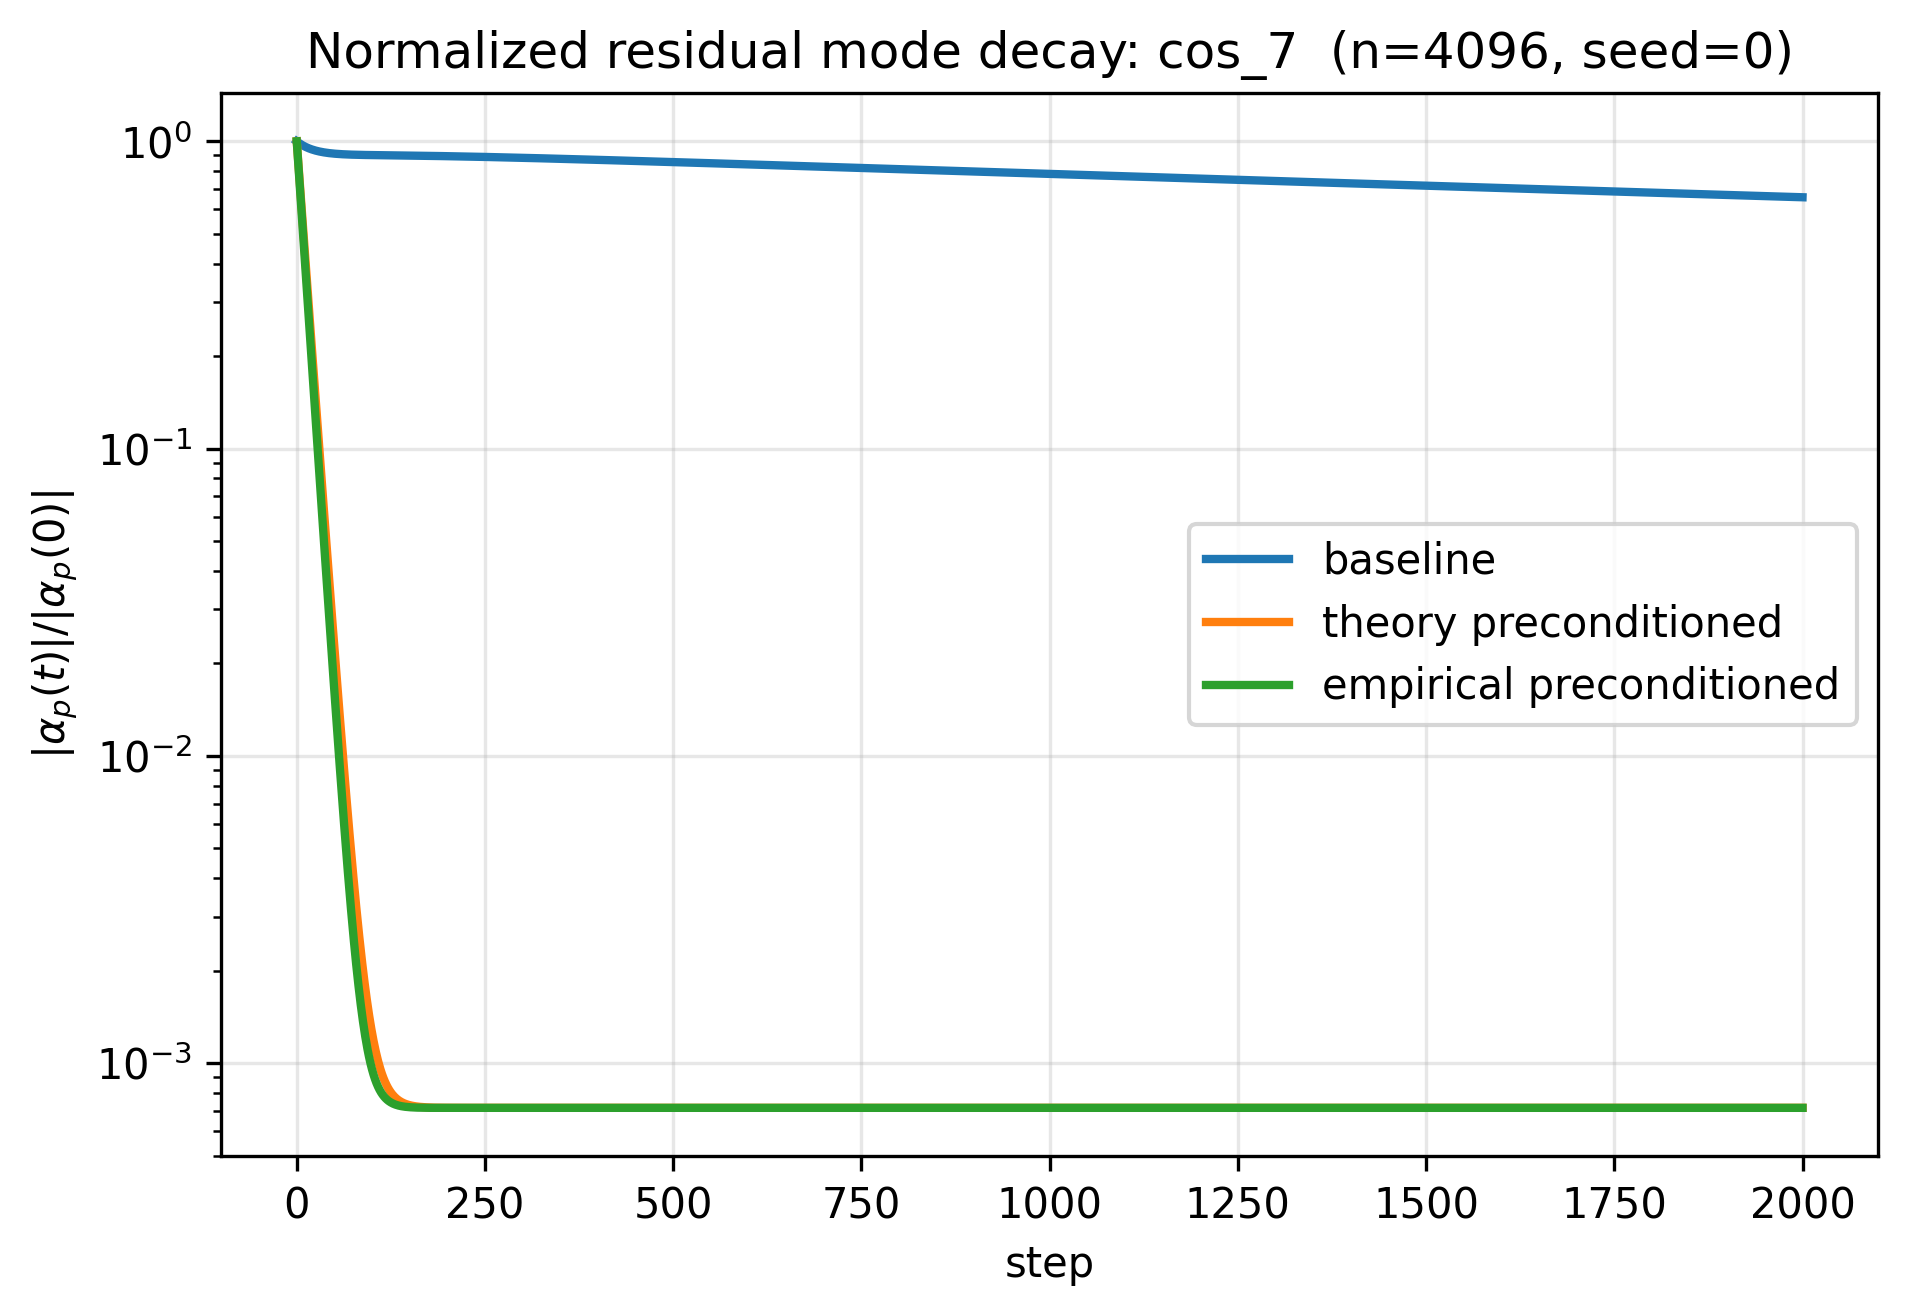
\includegraphics[width=\linewidth]{images/target-high-frequency/mode_curve_compare_cos_7_n4096_seed0.png}
		\caption{$\cos(7\gamma)$}
	\end{subfigure}
	\hfill
	\begin{subfigure}[t]{0.48\textwidth}
		\centering
		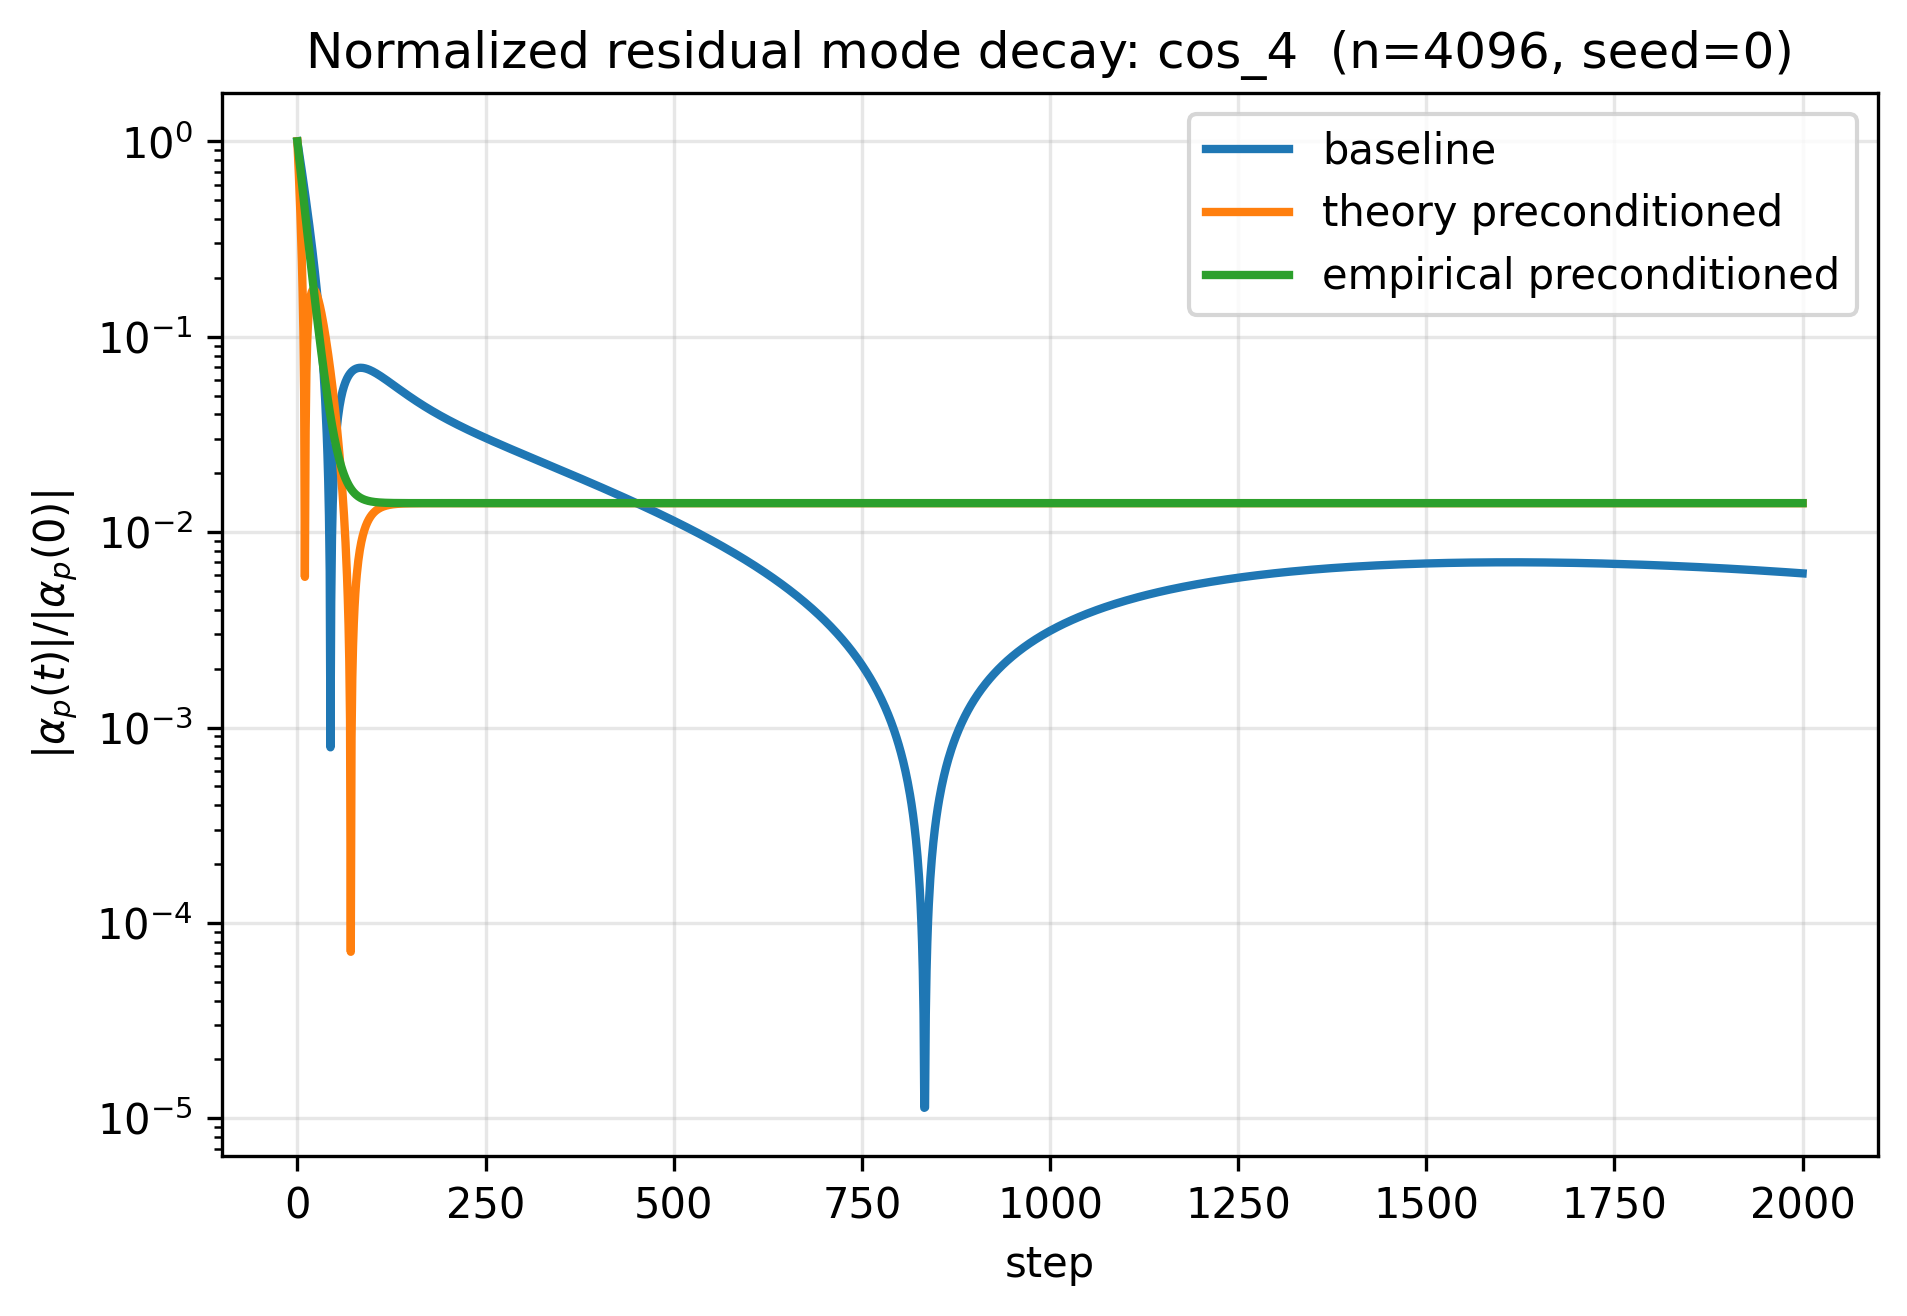
\includegraphics[width=\linewidth]{images/target-high-frequency/mode_curve_compare_cos_4_n4096_seed0.png}
		\caption{$\cos(4\gamma)$ (inactive in target)}
	\end{subfigure}

	\caption{Mixed/high-frequency target. Representative single-run mode comparisons at $n=4096$. The baseline separates the retained modes strongly, while the theory and empirical preconditioners again stay close to each other and make the retained-mode dynamics much more similar.}
\end{figure}

\end{document}
